\section[M5: Sirius]{M5: Sirius - grafischer Editor}
\begin{frame}{Sirius - grafischer Editor}
	\vspace{-5mm}
	\begin{columns}
		\column{.5\textwidth}
		\begin{contentblock}{}
			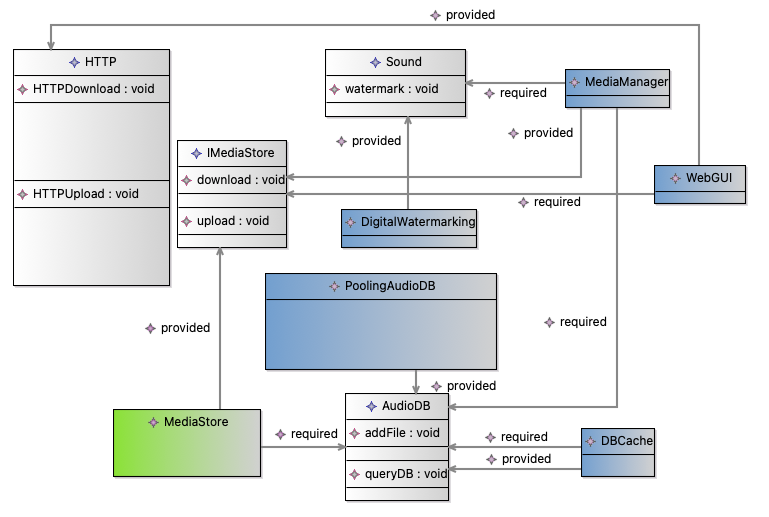
\includegraphics[width=86mm]{figures/sirius.png}
		\end{contentblock}
		\column{.5\textwidth}
		\begin{contentblock}{}
			\begin{itemize}
				\item graues Element: Interface
				\item grünes Element: Composite Component
				\item blaues Element: Component
				\item required Edge: z.B. Component required Interface 
				\item provided Edge: z.B. Component provided Interface
			\end{itemize}
		\end{contentblock}
	\end{columns}
\end{frame}

\begin{frame}{Entwurfsentscheidungen beim grafischen Editor}
	\begin{enumerate}
		\item Verwendung des grafischen Editors, um die Verwendung des Meta-Modells so intuiitiv wie möglich zu gestalten
		\begin{itemize}
			\item Verwendung von üblichen Farben, Symbolen, Icons ermöglicht die Modellierung von 
		\end{itemize}
		\item Parameter werden als Liste innerhalb von Signaturblöcken dargestellt
	\end{enumerate}
\end{frame}

\begin{frame}{Probleme beim grafischen Editor}
	\begin{enumerate}
		\item Kontextwechsel muss man wissen
		\begin{itemize}
			\item Beispiel: Signaturen gehören bei Sirius zu Interfaces $\rightarrow$ wenn Interface gelöscht wird, dann ist Signatur weg, in Meta-Modell ist es weiterhin da
		\end{itemize}
		\item Parameterlisten mit Klammern schwer umsetzbar, da sie nicht editierbar wäre
		\item eigenständige Datentypen als Parameter
	\end{enumerate}
\end{frame}